\documentclass[10pt]{ctexbeamer}
\usepackage{bm}
\usepackage{tikz}
\usepackage{amsmath}
\usepackage{graphicx}
\newfontfamily{\dengxian}{DengXian}
\newCJKfontfamily{\fzyaoti}{FZYaoTi} %方正姚体
\newCJKfontfamily{\fzjinghong}{FZZJ-JHTJW} %方正字迹-惊鸿体
\newCJKfontfamily{\dqheiti}{Hiragino Sans GB} %冬青黑体
\newCJKfontfamily{\fandolhei}{FandolHei}

% \usetheme[color blocks]{Verona}% 使用Verona主题
% \usetheme[color blocks, red]{Verona}% 使用Verona主题, red theme
% \usetheme[color blocks, gray]{Verona}% 使用Verona主题, grey theme
\usefonttheme[onlymath]{serif}% 数学公式字体设置
\author{Norsesun}
\date{最后更新:\today}
\logo{
\includegraphics[height=1.2cm]{../../../Pngtree owl double exposure.png}}

\definecolor{airforceblue}{rgb}{.36,.54,.66}



\newcommand{\bmc}[1]{$\bm{#1}$}%定义一个新命令,行内数学模式的粗体,使幻灯片上的公式更清楚
\newcommand{\bmcc}[1]{
        \begin{displaymath}
            \bm{#1}
        \end{displaymath}
    }%定义一个新命令,行间数学模式的粗体,使幻灯片上的公式更清楚
\newcommand{\makecenter}[1]{\vspace{0.5em}\centering \parbox{.6\textwidth}{#1}}%定义一个新命令,居中排布一段话
\newenvironment{Mathbreakcenter}[1][1mm]{
        \par
        \vspace{#1} 
        \centering

    }{
        \par
        \vspace{2mm}
    }
\newcommand{\myblock}[3][1-]{
    \centering
    \begin{minipage}{.6\textwidth}
        \begin{block}<#1>{#2}%
            \centering%
            #3
        \end{block}
    \end{minipage}  
    } %定义一个新命令,居中排布一个block

    \newcommand{\myalertblock}[3][1-]{
        \centering
        \begin{minipage}{.6\textwidth}
            \begin{alertblock}<#1>{#2}%
                \centering%
                #3
            \end{alertblock}
        \end{minipage}  
        } %定义一个新命令,居中排布一个alertblock
\newcommand{\cleave}[2]{
    \hbox to #1{} #2 \hbox to #1{}
}
% \newcommand{\annmark}[1]{%
%     \textcolor{red}{$\bm\langle$#1$\bm\rangle$}%
% }%

% \newcommand{\ann}[1]{%
%     \begin{tikzpicture}[remember picture, baseline=-0.75ex]%
%         \node[coordinate] (inText) {};%
%     \end{tikzpicture}%
%     \marginpar{%
%         \renewcommand{\baselinestretch}{1.0}%
%         \begin{tikzpicture}[remember picture]%
%             \definecolor{orange}{rgb}{1,0.5,0}%
%             \draw node[fill=red!20,rounded corners,text width=\marginparwidth] (inNote){\footnotesize#1};%
%     \end{tikzpicture}%
%     }%
%     \begin{tikzpicture}[remember picture, overlay]%
%         \draw[draw = orange, thick]
%             ([yshift=-0.2cm] inText)
%                 -| ([xshift=-0.2cm] inNote.west)
%                 -| (inNote.west);%
%     \end{tikzpicture}%
% }%

% \setlength{\marginparwidth}{2.5cm}
% \renewcommand{\baselinestretch}{1.3}

\newenvironment{mathsalvation}[2][{解:}]{
    \begin{center}{}
        \begin{minipage}[t]{.05\textwidth}
            \vspace{0pt}
            {\color{#2}{#1}} \quad 
        \end{minipage}
        \begin{minipage}[t]{.7\textwidth}
            \vspace{0pt}
            % \fzyaoti
            % \dengxian
            % \fzjinghong
            % \dqheiti
            \fandolhei
}{
    \end{minipage}
    \end{center}
}


\usepackage{array}

\title{建立一元一次方程模型}
\subtitle{Linear Equation with One Unknown}
\begin{document}
\frame{\titlepage}

\begin{frame}[t]
    \frametitle{新知导入}
    \begin{block}{列数学表达式}
        \begin{columns}
            \column{.49\textwidth}
            比b大8的数:\only<2->{\bmc{b+8}}

            \column{.49\textwidth}
            比b大8的数等于5: \only<2->{\bmc{b+8=5}}
        \end{columns}
    \end{block}
    \only<2->{
        \centering
        前者是代数式中的\alert{多项式},后者是一个\alert{方程}。\\
        那么什么是方程?
    }
        \begin{alertblock}<3->{方程(Equation)}
            含有未知数的等式叫做方程。
        \end{alertblock}

        \begin{columns}
            \column{0.49\textwidth}
            \only<3->{方程必须具备的两个条件:}
            \begin{enumerate}
                \item<3-> 是等式
                \item<3-> 含有未知数
            \end{enumerate}
            \column{0.49\textwidth}<4>
            % \begin{figure}
                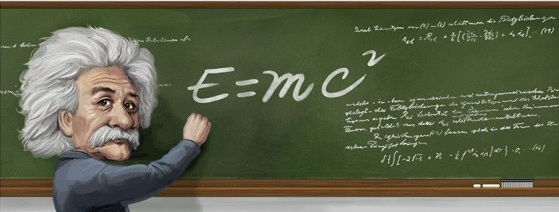
\includegraphics[width=.99\textwidth]{assets/equation of albert.jpg}
            % \end{figure}
            \parbox{.75\textwidth}{\zihao{6}{
            质能方程(Mass–Energy Equivalence),世界上最著名的方程之一。
            它看上去那么简洁,
            却给了人无限的想象空间,原来质量和能量是可以互相转换的。}}
        \end{columns}
\end{frame}

\begin{frame}{学什么?}
    \begin{figure}
        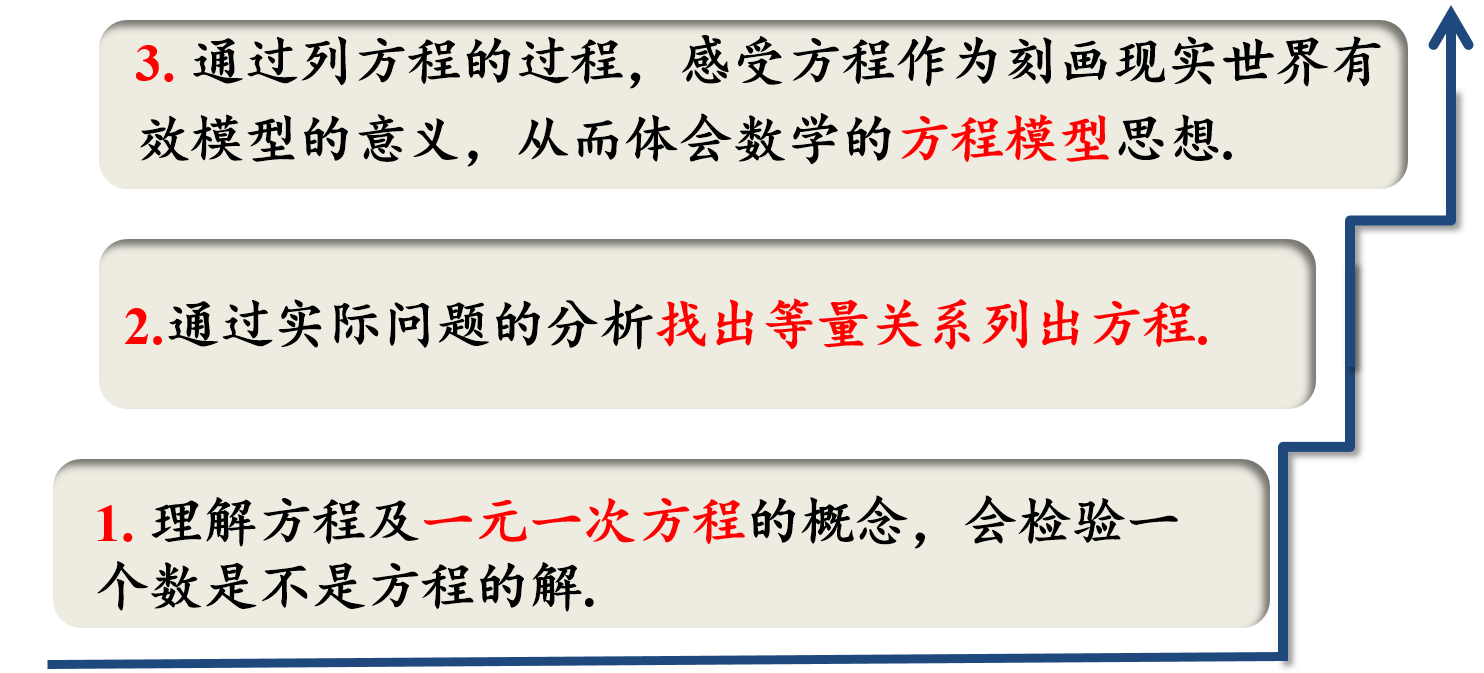
\includegraphics[width=.9\textwidth]{assets/equation teaching.png}
    \end{figure}
\end{frame}

\begin{frame}{列算式与列方程}
    汽车匀速行驶途径王家庄、青山、秀水三地的时间如表所示,翠湖在青山、秀水
    两地之间,距青山50千米,距秀水70千米。王家庄到翠湖的路程有多远?
    \begin{table}
        \setlength{\extrarowheight}{1.5pt}
        \begin{tabular}{ll}
            地名 & 时间 \\
            \hline
            王家庄 & $10:00$ \\
            \hline
            青山 & $13:00$ \\
            \hline
            秀水 & $15:00$ \\
            \hline
        \end{tabular}
    \end{table}

    \begin{figure}
        \includegraphics<2>[width=.9\textwidth]{assets/equation examp2.png}
    \end{figure}

    \begin{figure}
        \includegraphics<3>[width=.7\textwidth]{assets/equation examp3.png}
    \end{figure}
\end{frame}

\begin{frame}
    \only<1->{\begin{figure}
        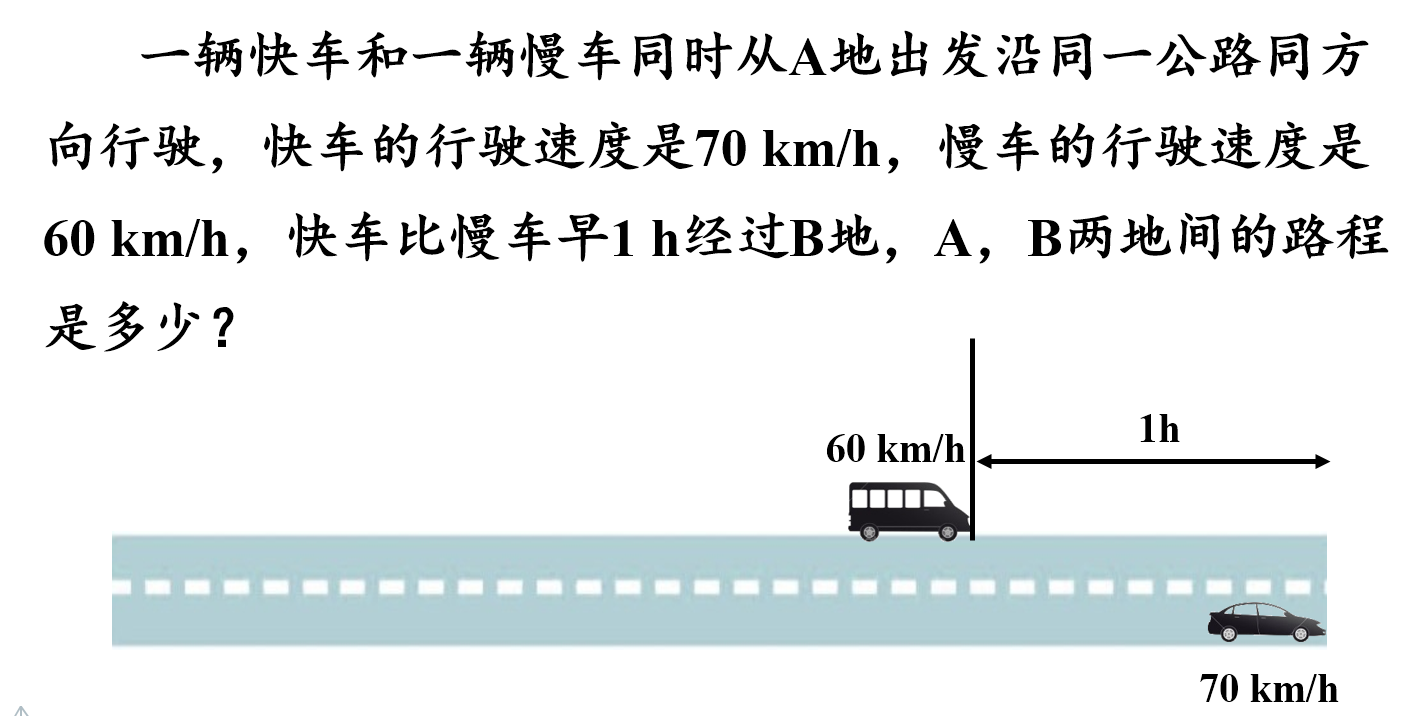
\includegraphics[width=.75\textwidth]{assets/equation.png}
    \end{figure}}
    \begin{columns}
        \column{.65\textwidth}
        \only<2>{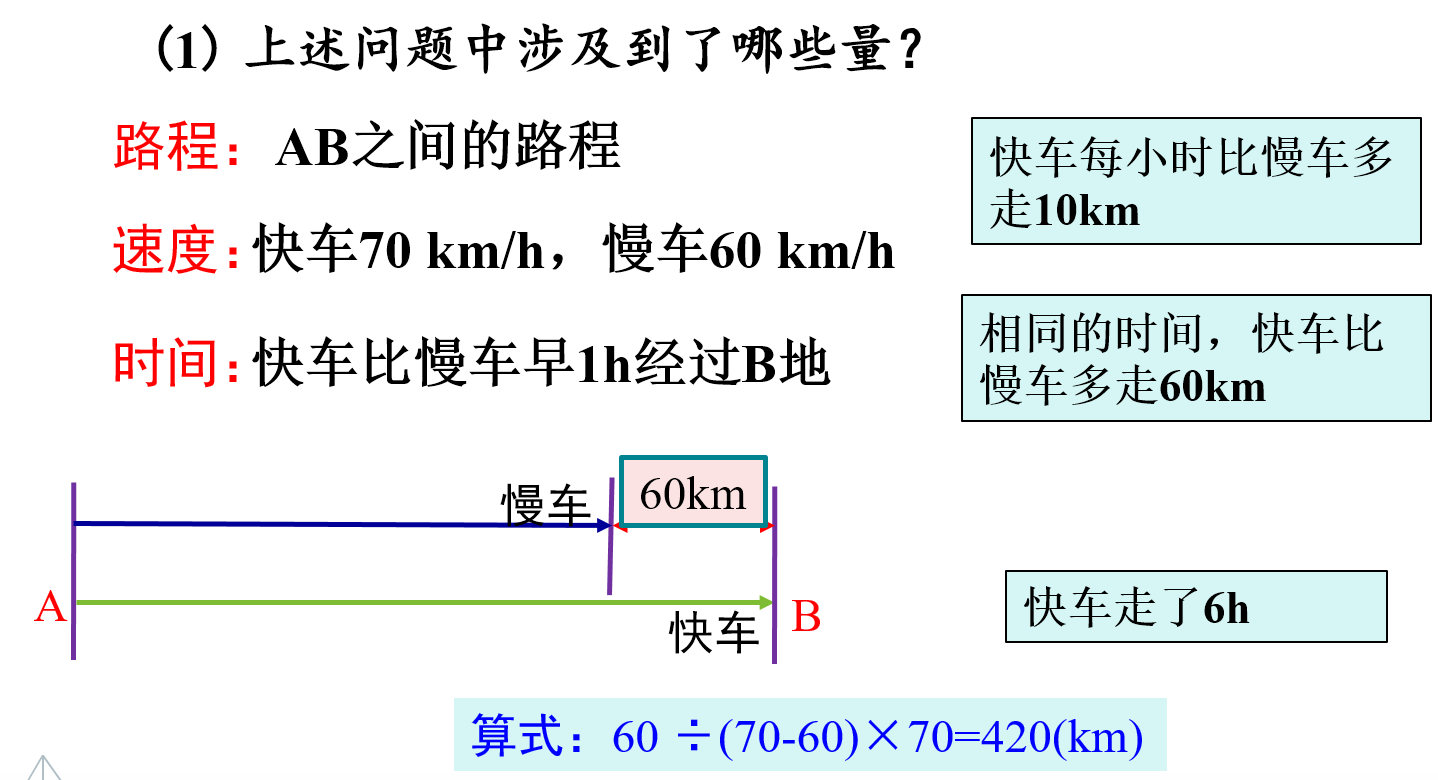
\includegraphics[width=.99\textwidth]{assets/equation examp4.png}}
        \only<3>{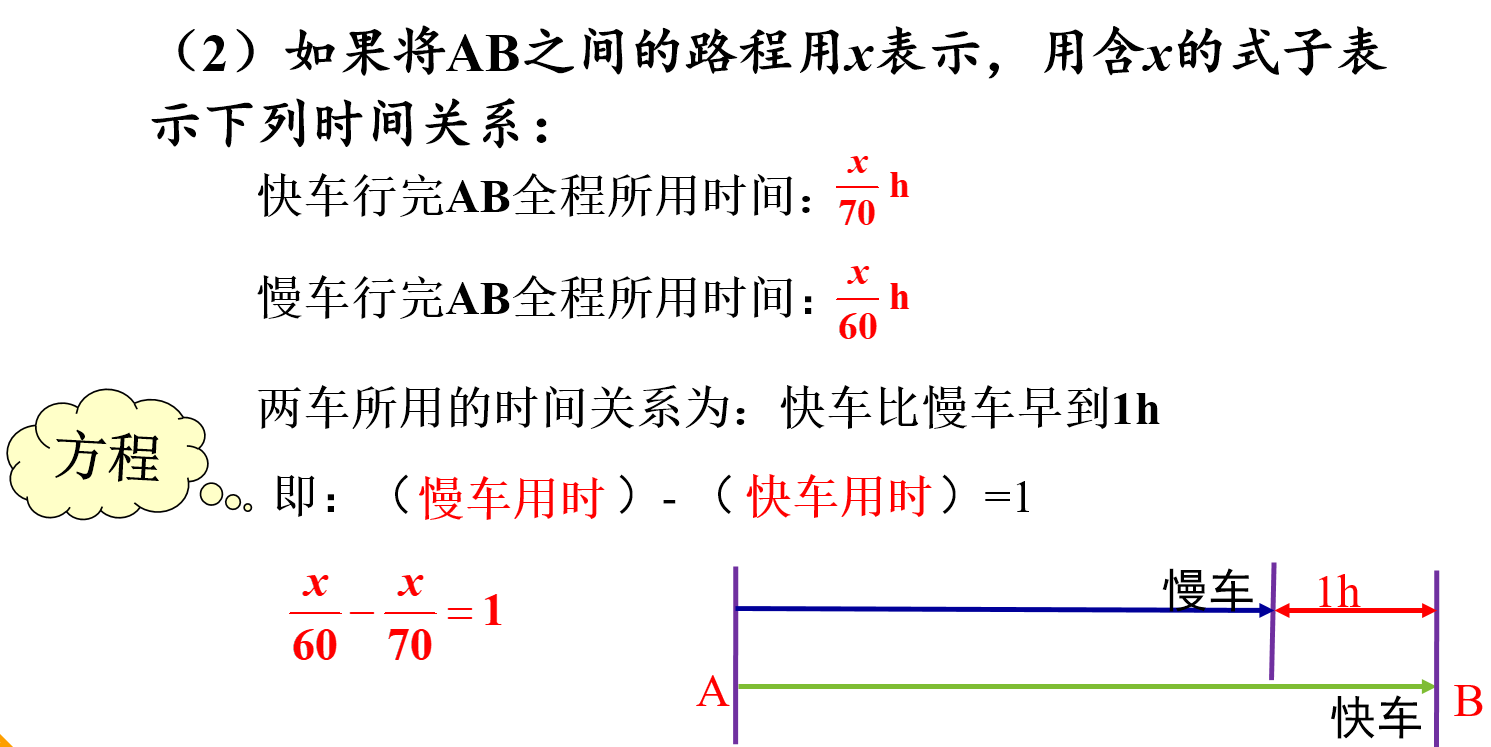
\includegraphics[width=.99\textwidth]{assets/equation examp5.png}}
        \includegraphics<4>[width=.99\textwidth]{assets/equation examp6.png}
        \includegraphics<5>[width=.99\textwidth]{assets/equation examp7.png}
    \end{columns}
\end{frame}
\begin{frame}{对比}
    \begin{figure}
        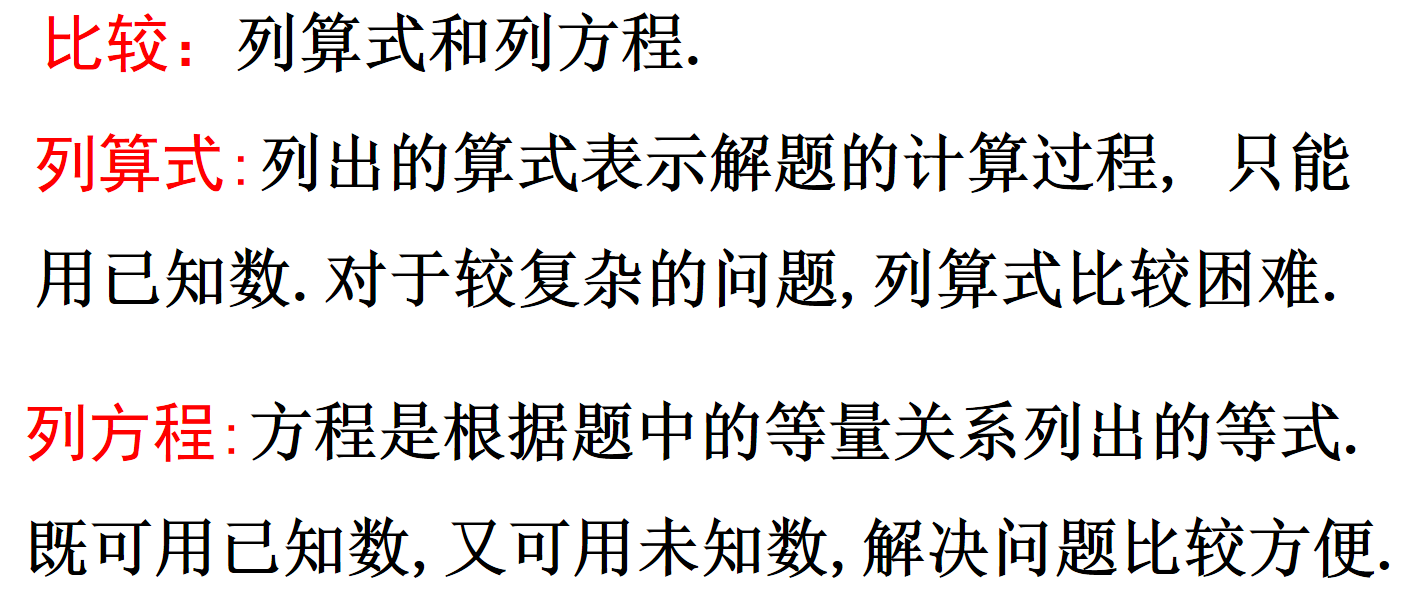
\includegraphics[width=.9\textwidth]{assets/comparison.png}
    \end{figure}
\end{frame}

\begin{frame}{新概念}
    \begin{figure}
        \includegraphics<1>[width=.9\textwidth]{assets/new.png}
        \includegraphics<2>[width=.9\textwidth]{assets/new2.png}
    \end{figure}
\end{frame}

\begin{frame}{新概念:一元一次方程}{Equation with one Unknown}
    \begin{figure}
        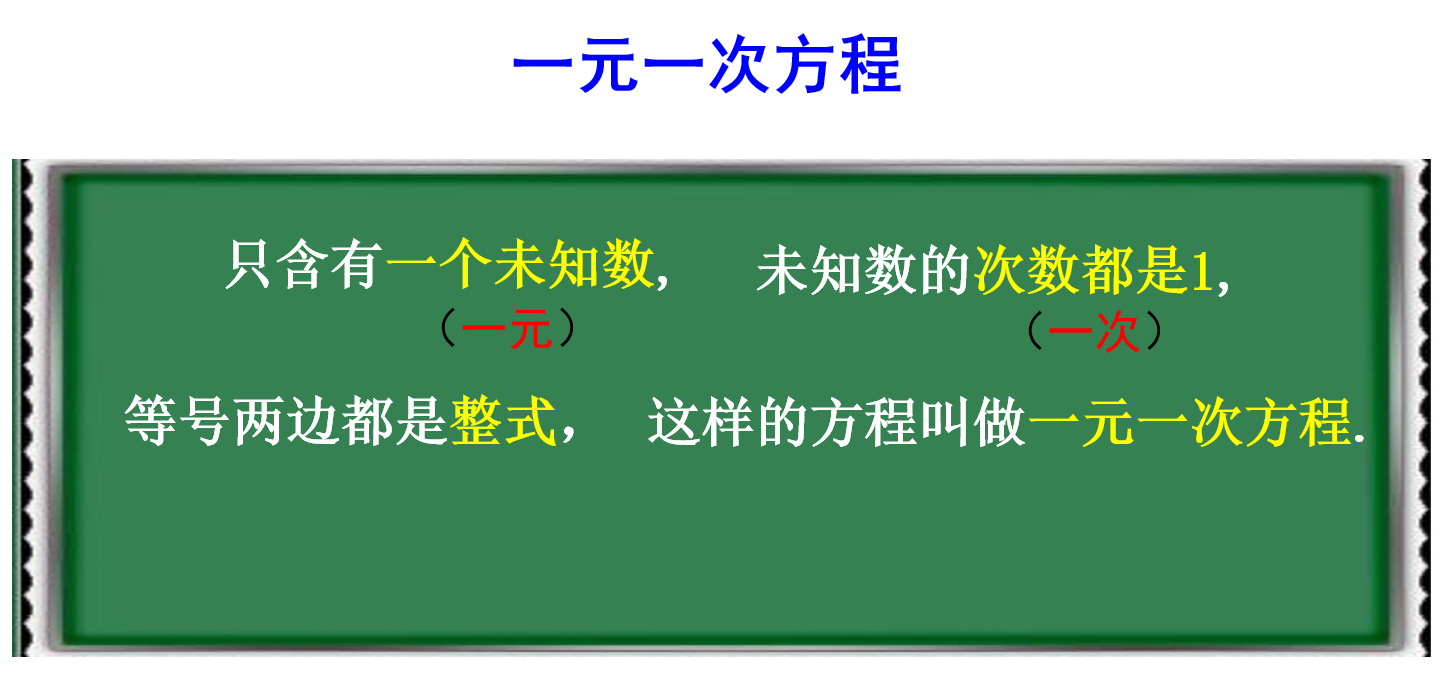
\includegraphics[width=.9\textwidth]{assets/new3.png}
    \end{figure}
\end{frame}

\begin{frame}{辨别一元一次方程}
    \begin{figure}
        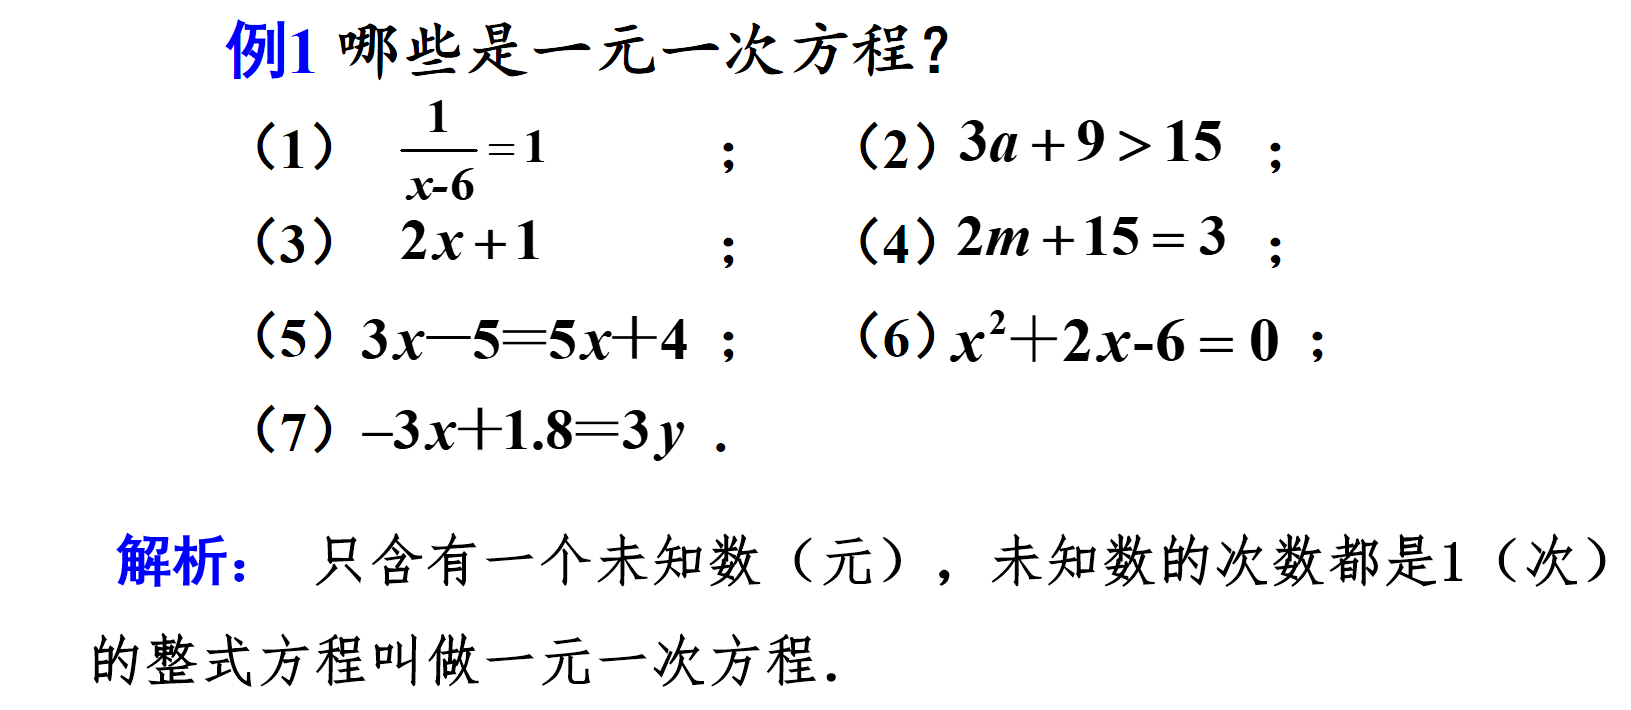
\includegraphics[width=.9\textwidth]{assets/new4.png}
    \end{figure}
\end{frame}

\begin{frame}{一元一次方程变式题}
    \begin{figure}
        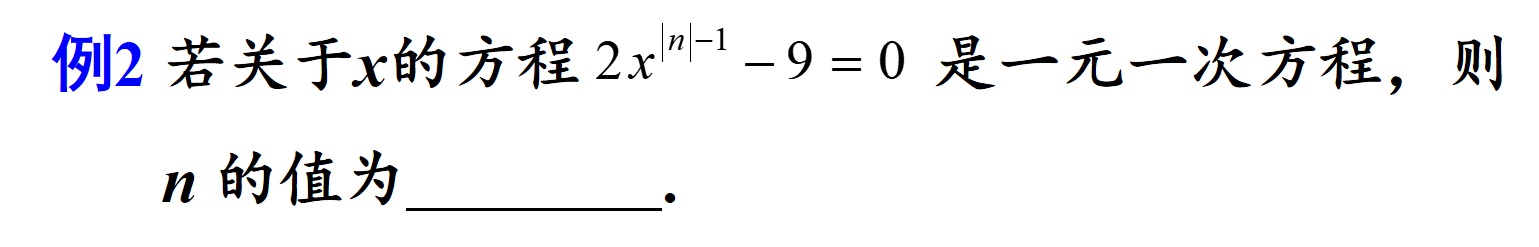
\includegraphics[width=.9\textwidth]{assets/new5.png}
    \end{figure}

    \begin{block}{}
        已知方程 \bmc{(m-2)x^{|m|-1} +3 = m -5}是关于 $x$的一
        元一次方程,求$m$的值,并写出其方程。
    \end{block}
\end{frame}

\begin{frame}{一元一次方程的应用}
    \begin{figure}
        \includegraphics<1>[width=.9\textwidth]{assets/new6.png}
        \includegraphics<2>[width=.9\textwidth]{assets/new7.png}

    \end{figure}
\end{frame}

\begin{frame}{一元一次方程的应用}
    \begin{figure}
        \includegraphics<1>[width=.9\textwidth]{assets/new8.png}
    \end{figure}
\end{frame}

\begin{frame}{一元一次方程的应用}
    \begin{figure}
        \includegraphics<1>[width=.9\textwidth]{assets/new9.png}
        \includegraphics<2>[width=.9\textwidth]{assets/new10.png}

    \end{figure}
\end{frame}

\begin{frame}
    \begin{block}{选择}
        由于受禽流感的影响,我市某城区今年2月份鸡的价格比1月份下降a\%,
        3月份比2月份下降b\%,已知1月份鸡的价格为24元/千克。
        设3月份鸡的价格为m元/千克,则( )\\
        A. $m=24(1-a\%-b\%)$          \\
        B. $m=24(1-a\%)b\%$\\
        C. $m=24-a\%-b\%$            \\    
        D. $m=24(1-a\%)(1-b\%)$

    \end{block}
\end{frame}

\begin{frame}{方程的解}
    \begin{figure}
        \includegraphics<1>[width=.9\textwidth]{assets/solution.png}
        \includegraphics<2>[width=.9\textwidth]{assets/solution2.png}
    \end{figure}
\end{frame}

\begin{frame}{方程的解}
    \begin{block}{\bmc{x=3}是不是下列方程的解?\bmc{x=4,5,6}时呢?}
        \bmc{2x-3=5x-15}
    \end{block}
    \includegraphics<2>[width=.5\textwidth]{assets/solution3.png}
\end{frame}

\begin{frame}
    \begin{block}{}
        若关于 $x$的方程 \bmc{2x+a=x-1}的解是 \bmc{x=-2},求\bmc{a^{2018}}的值。
    \end{block}
\end{frame}

\begin{frame}{如何判断方程的解}
    \begin{figure}
        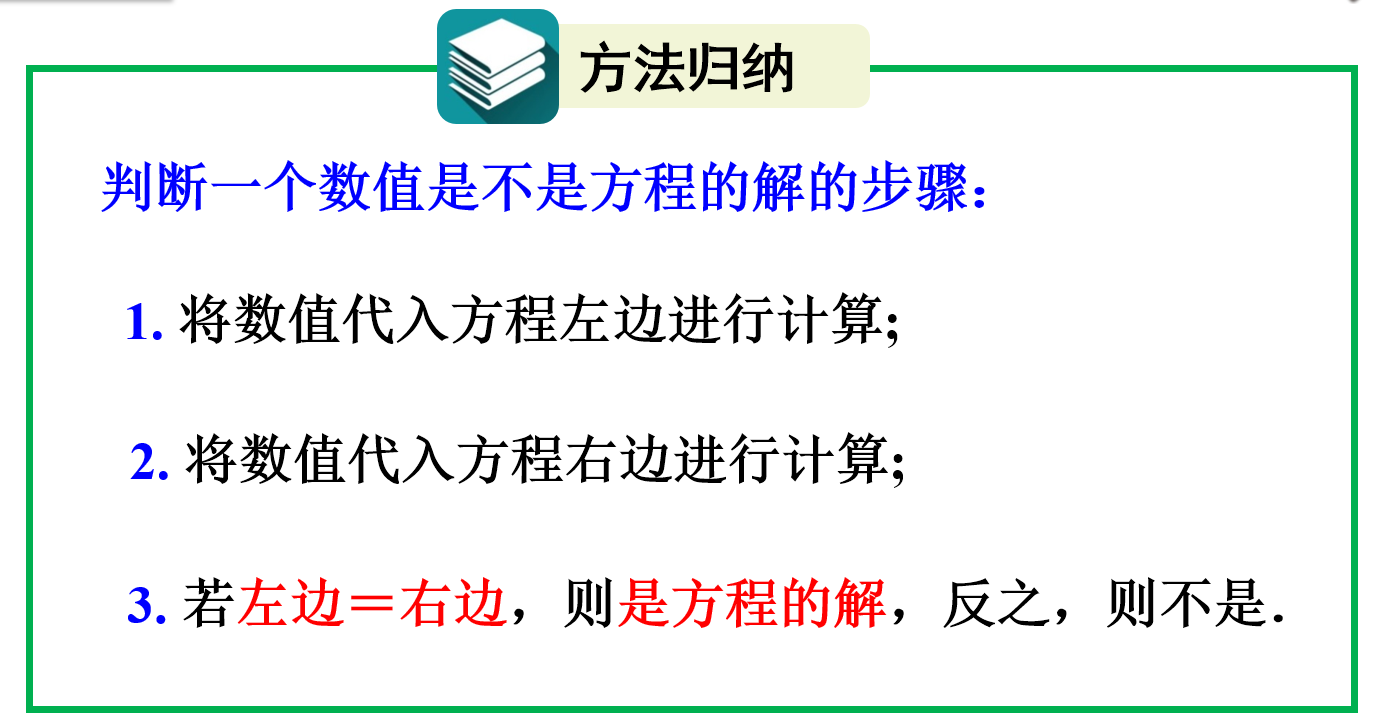
\includegraphics[width=.9\textwidth]{assets/solutions.png}
    \end{figure}
\end{frame}

\begin{frame}{总结(Overview)}
    \begin{figure}
        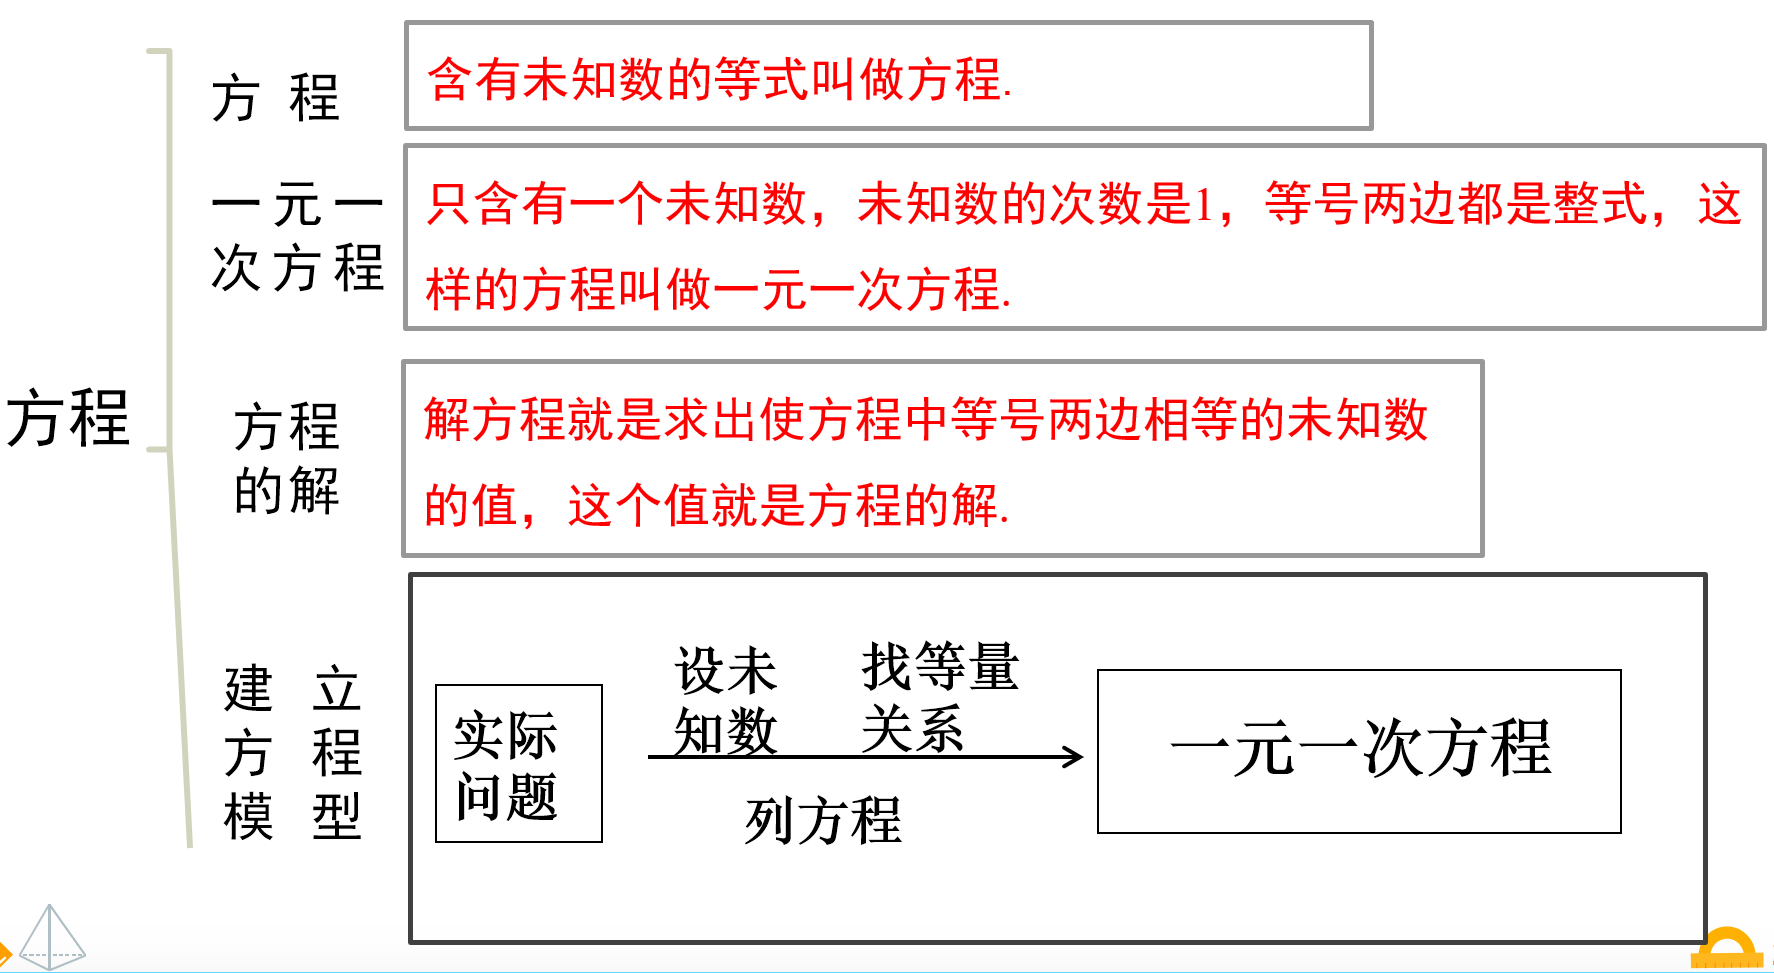
\includegraphics[width=.99\textwidth]{assets/overview.png}
    \end{figure}
\end{frame}

\setbeamercolor{background canvas}{bg=airforceblue}
\begin{frame}[plain]
    \centering
    \begin{quote}
        \Large 方程式对我更重要,因为政治只看眼前,而方程式是永恒的\footnote{Equation are more important to me, because politics is for the present, but an equation is something for eternity.}。\\
        \raggedleft
        ——爱因斯坦
    \end{quote}
    \titlegraphic[scale=0.6]{assets/Einstein.jpg}{}
\end{frame}
\end{document}